\documentclass{article}
\usepackage{graphicx} % Required for inserting images
\usepackage{tikz} % Drawing
\usepackage[backend=biber,style=apa]{biblatex}
\usepackage{amsmath}

% load bib
\addbibresource{reference.bib}

\title{BKT}
\author{Yuhao Yuan, Biying Zhou, Feng Ji}
\date{\today}

\begin{document}

\maketitle

\section{Introduction}


\section{Model description}

\subsection{Bayesian Knowledge Tracing}
BKT (Bayesian Knowledge Tracing) is a probabilistic model designed to track a learner’s state of knowledge over time, specifically focusing on transitions between 'unknown' and 'known' states for a particular skill or concept. BKT assumes that a learner has a probability of transitioning from an unknown state to a known state based on the correctness of their responses during learning activities. Here, we provide detailed explanations of the learning process as abstracted by the BKT model.

In general, people acquire knowledge by engaging in learning activities. Learner's knowledge state can be observed by changes in their performance on these activities. This learning process is illustrated in Figure 1.

\begin{center}
    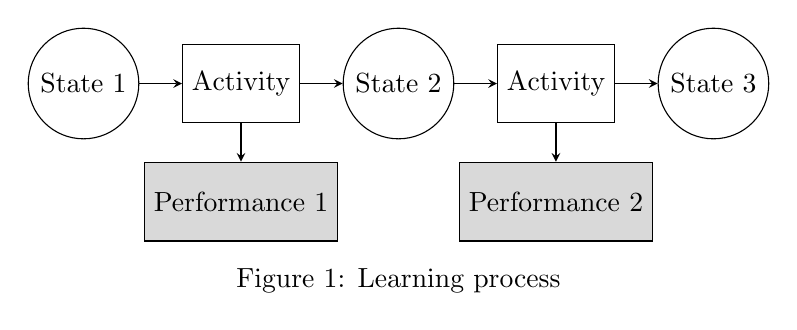
\begin{tikzpicture}
        % Define styles
        \tikzset{
            state/.style={circle, draw, minimum size=1cm},
            activity/.style={rectangle, draw, minimum size=1cm},
            performance/.style={rectangle, draw, fill=gray!30, minimum size=1cm},
            arrow/.style={->,>=stealth}
        }
        
        % Nodes
        \node[state] (state_node_1) at (0,0) {State 1};
        \node[activity] (activity_node_1) at (2,0) {Activity};
        \node[performance] (performance_node_1) at (2,-1.5) {Performance 1};
        \node[state] (state_node_2) at (4,0) {State 2};
        
        \node[activity] (activity_node_2) at (6,0) {Activity};
        \node[performance] (performance_node_2) at (6,-1.5) {Performance 2};
        \node[state] (state_node_3) at (8,0) {State 3};
        
        % Arrows
        \draw[arrow] (state_node_1) -- (activity_node_1);
        \draw[arrow] (activity_node_1) -- (state_node_2);
        \draw[arrow] (activity_node_1) -- (performance_node_1);
        \draw[arrow] (state_node_2) -- (activity_node_2);
        \draw[arrow] (activity_node_2) -- (state_node_3);
        \draw[arrow] (activity_node_2) -- (performance_node_2);
    
        % Footnote
        \node at (4,-2.5) {Figure 1: Learning process};
    \end{tikzpicture}
\end{center}

Another assumption of the BKT model is the binary nature of learning states and the impact of activities on these states. BKT assumes that a learner is either in a known state or an unknown state. By participating in an activity, a learner in the unknown state has a chance to transition to the known state. Therefore, learning activities cause three types of state changes: remaining known, learning (transitioning from unknown to known), and remaining unknown. This is illustrated in Figure 2. Note that the transition from the unknown state to the known state represents the learning process as a hidden Markov model in the BKT framework.

\begin{center}
    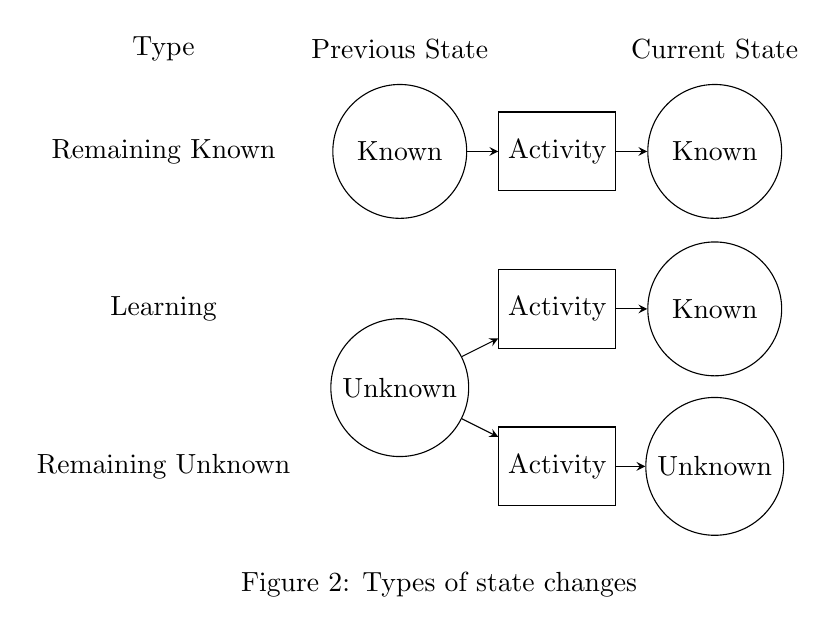
\begin{tikzpicture}
        % Define styles
        \tikzset{
            state/.style={circle, draw, minimum size=1.7cm},
            activity/.style={rectangle, draw, minimum size=1cm},
            arrow/.style={->,>=stealth}
        }
        
        % Nodes
        \node[] () at (-3,1.3) {Type};
        \node[] () at (0,1.3) {Previous State};
        \node[] () at (4,1.3) {Current State};

        \node[] () at (-3,0) {Remaining Known};
        \node[state] (state_node_1) at (0,0) {Known};
        \node[activity] (activity_node_1) at (2,0) {Activity};
        \node[state] (state_node_2) at (4,0) {Known};
        
        \node[] () at (-3,-2) {Learning};
        \node[state] (state_node_3) at (0,-3) {Unknown};
        \node[activity] (activity_node_2) at (2,-2) {Activity};
        \node[state] (state_node_4) at (4,-2) {Known};
        
        \node[] () at (-3,-4) {Remaining Unknown};
        % \node[state] (state_node_5) at (0,-4) {Unknown};
        \node[activity] (activity_node_3) at (2,-4) {Activity};
        \node[state] (state_node_6) at (4,-4) {Unknown};
        
        % Arrows
        \draw[arrow] (state_node_1) -- (activity_node_1);
        \draw[arrow] (activity_node_1) -- (state_node_2);
        \draw[arrow] (state_node_3) -- (activity_node_2);
        \draw[arrow] (activity_node_2) -- (state_node_4);
        \draw[arrow] (state_node_3) -- (activity_node_3);
        \draw[arrow] (activity_node_3) -- (state_node_6);
    
        % Footnote
        \node at (0.5,-5.5) {Figure 2: Types of state changes};
    \end{tikzpicture}
\end{center}

One can infer a learner’s knowledge state by observing their performance on activities. However, there are two common scenarios to consider: a learner in an unknown state answering correctly (guessing) and a learner in a known state answering incorrectly (slipping). The relationship between activity performance and knowledge state is shown in Figure 3.

\begin{center}
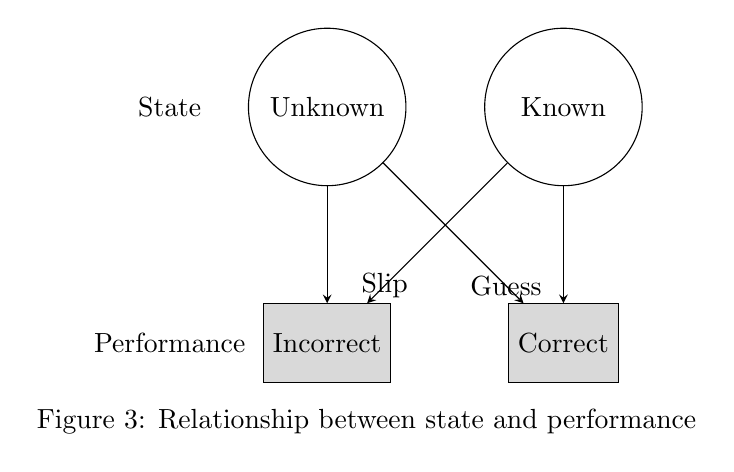
\begin{tikzpicture}
    % Define styles
    \tikzset{
        state/.style={circle, draw, minimum size=2cm},
        performance/.style={rectangle, draw, fill=gray!30, minimum size=1cm},
        arrow/.style={->,>=stealth}
    }
    
    % Nodes
    \node[] (state_label) at (-1,0) {State};
    \node[] (performance_label) at (-1,-3) {Performance};
    \node[state] (not_known) at (1,0) {Unknown};
    \node[state] (known) at (4,0) {Known};
    \node[performance] (incorrect) at (1,-3) {Incorrect};
    \node[performance] (correct) at (4,-3) {Correct};
    
    % Arrows
    \draw[arrow] (not_known) -- (incorrect);
    \draw[arrow] (not_known) -- (correct) node[very near end] {Guess};
    \draw[arrow] (known) -- (correct);
    \draw[arrow] (known) -- (incorrect) node[very near end] {Slip};

    % Footnote
    \node at (1.5,-4) {Figure 3: Relationship between state and performance};
\end{tikzpicture}
\end{center}

BKT provides a static approach, using specific and quantified probability descriptions to calculate the likelihood of the learning process.

In BKT terminology, we define the following:

1. \textbf{Answer}  
The answer for an activity, denoted as \( a \), represents the response given by a learner during the activity. According to BKT assumptions, its value is binary, either 0 or 1.

The variable \textbf{Answer} is the only input variable in this model.

2. \textbf{Prior}  
The prior rate, \( P_p \), represents the probability that a learner is initially in the known state.

3. \textbf{Learn}  
The learning rate, \( P_l \), indicates the probability that a learner transitions to the known state through learning.

4. \textbf{Slip}  
The slip rate, \( P_s \), denotes the probability that a learner in the known state answers incorrectly.

5. \textbf{Guess}  
The guess rate, \( P_g \), represents the probability that a learner in the unknown state answers correctly.

These four variables (\textbf{Prior} \textbf{Learn} \textbf{Slip} \textbf{Guess}) are global parameters that remain constant throughout the model.

6. \textbf{Know}  
The known rate, \( \theta \), reflects the probability that a learner is in the known state. Unlike the other parameters, \textbf{Know} is dynamic and updates iteratively as the model progresses.

For a learning process with an answer vector \( (a_1, a_2, \dots, a_s) \), the likelihood of the sequence in the BKT model is calculated as follows:

For each answer \( a_i \), let \(\theta_{i}\) denote the known rate before the \(i\)-th activity, and \(\theta_{i+1}\) the known rate after the \(i\)-th activity. Note \(\theta_1 = P_p\). The iteration of \(\theta_{i+1}\) is as follows:

First, calculate \(\theta'\), the updated known rate using Bayes' rule based on the observed answer \( a_i \):
\[
\theta' = 
\begin{cases} 
    \frac{\theta_{i} P_s}{\theta_{i} P_s + (1 - \theta_{i}) (1 - P_g)}, & \text{if } a_i = 0 \\[10pt]
    \frac{\theta_{i} (1 - P_s)}{\theta_{i} (1 - P_s) + (1 - \theta_{i}) P_g}, & \text{if } a_i = 1 
\end{cases}
\]

Figure 4 illustrates the Bayes update process.

\begin{center}
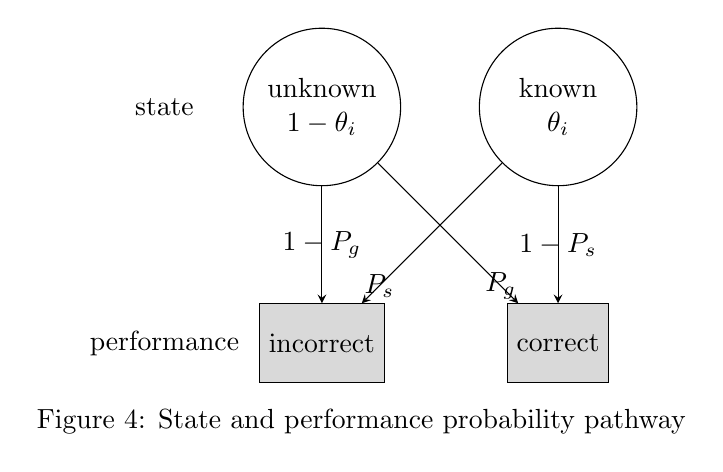
\begin{tikzpicture}
    % Define styles
    \tikzset{
        state/.style={circle, draw, minimum size=2cm},
        performance/.style={rectangle, draw, fill=gray!30, minimum size=1cm},
        arrow/.style={->,>=stealth}
    }
    
    % Nodes
    \node[] (state_node) at (-1,0) {state};
    \node[] (performance_node) at (-1,-3) {performance};
    \node[state] (not_known) at (1,0) {\parbox{1.5cm}{\centering unknown \\ \(1 - \theta_i\)}};
    \node[state] (known) at (4,0) {\parbox{1.5cm}{\centering known \\ \(\theta_{i}\)}};
    \node[performance] (incorrect) at (1,-3) {incorrect};
    \node[performance] (correct) at (4,-3) {correct};
    
    % Arrows
    \draw[arrow] (not_known) -- (incorrect) node[midway] {$1 - P_g$};
    \draw[arrow] (not_known) -- (correct) node[very near end] {$P_g$};
    \draw[arrow] (known) -- (correct) node[midway] {$1 - P_s$};
    \draw[arrow] (known) -- (incorrect) node[very near end] {$P_s$};

    % Figure label
    \node at (1.5,-4) {Figure 4: State and performance probability pathway};
\end{tikzpicture}
\end{center}

Then, update \(\theta_{i+1}\) by incorporating the potential learning effect based on \(\theta'\).

\[
\theta_{i+1} = \theta' + (1 - \theta') P_l    
\]

Now we know all learn rate before each activity \(\theta_i\), we use them to calculate the probability of each activity outcome.

\[
    Lik_i = 
    \begin{cases} 
        P_s \theta_{i} + (1 - P_g) (1 - \theta_i), & \text{if } a_i = 0 \\[10pt]
        (1 - P_s) \theta_{i} + P_g (1 - \theta_i), & \text{if } a_i = 1 
    \end{cases}
\]

So the total learn process's probability is

\[
    Lik = \prod Lik_i
\]

We can utilize the standard expectation-maximization algorithm to determine the global parameters (\(P_p, P_l, P_s, P_g\))

The basic Bayesian Knowledge Tracing (BKT) model is involved here. However, it should be noted that the basic BKT model has certain limitations. The most significant issue is that it presupposes a large number of global parameters. As a result of applying these global parameters to local scenarios, numerous variants of the BKT model have emerged. At the same time, by expanding the functionality of the BKT model, some variant BKT models have also been proposed.

\subsection{BKT Variants}

% variant              name                                                        url              
% forget               Knowledge Tracing and Forgets Models                https://dl.acm.org/doi/abs/10.1145/3511808.3557622
% multilearn         Item Learning Effect Model                            http://ml4ed.cc/attachments/XuY.pdf
% multiguess        Item Difficulty Effect Mode                            https://link.springer.com/chapter/10.1007/978-3-642-22362-4_21
% multiprior          Prior per Student Model                              https://link.springer.com/chapter/10.1007/978-3-642-13470-8_24
% multipair           Item Order Effect Model                              https://eric.ed.gov/?id=ED539081
% fixed
Before introducing variants, we need to know how the basic BKT handles learning processes of multiple students.

In general, BKT calculate each student learning process likelihood individually while using same global parameters as shown in Figure 5.

\begin{center}
    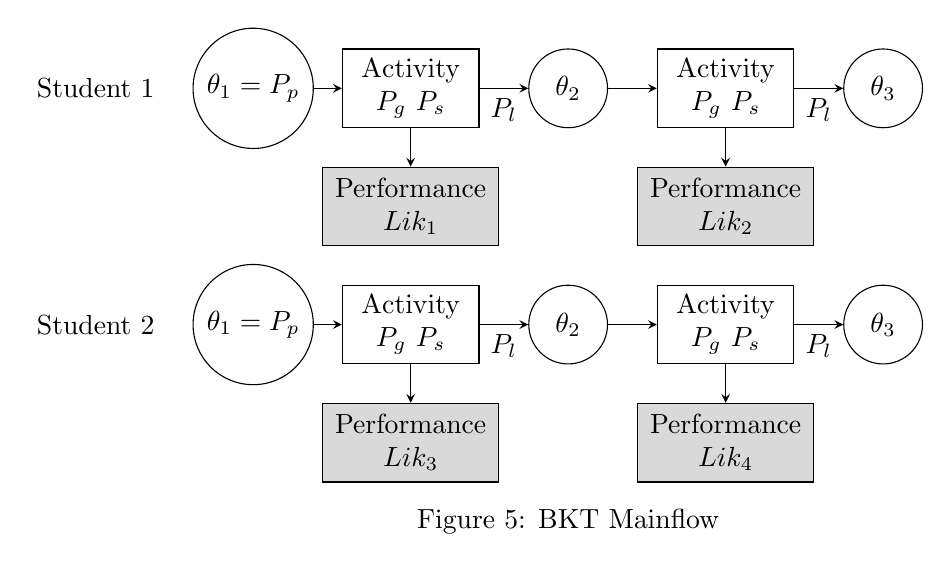
\begin{tikzpicture}
        % Define styles
        \tikzset{
            state/.style={circle, draw, minimum size=1cm},
            activity/.style={rectangle, draw, minimum size=1cm},
            performance/.style={rectangle, draw, fill=gray!30, minimum size=1cm},
            arrow/.style={->,>=stealth}
        }
        
        % Nodes
        \node[] () at (-2,0) {Student 1};
        \node[state] (state_node_1) at (0,0) {$\theta_1 = P_p$};
        \node[activity] (activity_node_1) at (2,0) {\parbox{1.5cm}{\centering Activity \\ $P_g \ P_s$}};
        \node[performance] (performance_node_1) at (2,-1.5) {\parbox{2cm}{\centering Performance \\ $Lik_1$}};
        \node[state] (state_node_2) at (4,0) {$\theta_2$};
        
        \node[activity] (activity_node_2) at (6,0) {\parbox{1.5cm}{\centering Activity \\ $P_g \ P_s$}};
        \node[performance] (performance_node_2) at (6,-1.5) {\parbox{2cm}{\centering Performance \\ $Lik_2$}};
        \node[state] (state_node_3) at (8,0) {$\theta_3$};
        
        % Arrows
        \draw[arrow] (state_node_1) -- (activity_node_1);
        \draw[arrow] (activity_node_1) -- (state_node_2) node[midway, below] {$P_l$};
        \draw[arrow] (activity_node_1) -- (performance_node_1);
        \draw[arrow] (state_node_2) -- (activity_node_2);
        \draw[arrow] (activity_node_2) -- (state_node_3) node[midway, below] {$P_l$};
        \draw[arrow] (activity_node_2) -- (performance_node_2);
    

        % student 2
        \node[] () at (-2,-3) {Student 2};
        \node[state] (state_node_2) at (0,-3) {$\theta_1 = P_p$};
        \node[activity] (activity_node_2) at (2,-3) {\parbox{1.5cm}{\centering Activity \\ $P_g \ P_s$}};
        \node[performance] (performance_node_2) at (2,-4.5) {\parbox{2cm}{\centering Performance \\ $Lik_3$}};
        \node[state] (state_node_3) at (4,-3) {$\theta_2$};
        \node[activity] (activity_node_3) at (6,-3) {\parbox{1.5cm}{\centering Activity \\ $P_g \ P_s$}};
        \node[performance] (performance_node_3) at (6,-4.5) {\parbox{2cm}{\centering Performance \\ $Lik_4$}};
        \node[state] (state_node_4) at (8,-3) {$\theta_3$};
        \draw[arrow] (state_node_2) -- (activity_node_2);
        \draw[arrow] (activity_node_2) -- (state_node_3) node[midway, below] {$P_l$};
        \draw[arrow] (activity_node_2) -- (performance_node_2);
        \draw[arrow] (state_node_3) -- (activity_node_3);
        \draw[arrow] (activity_node_3) -- (state_node_4) node[midway, below] {$P_l$};
        \draw[arrow] (activity_node_3) -- (performance_node_3);

        % Footnote
        \node at (4,-5.5) {Figure 5: BKT Mainflow};
    \end{tikzpicture}
\end{center}

\subsubsection{Multiple Prior}
The Prior Per Student (PPS) Model (\cite{multiprior}) is based on BKT that focuses on individualizing the prior. The BKT assumes all student share same prior rate, the global parameter \( P_p \). The PPS localizes prior rate into each student.

The main difference in the model description lies in the initial known rate.

For each student \( j \), let \( P_{p_j} \) denote their individual prior rate. Let \(\theta_{i_j}\) denote the known rate before the \(i\)-th activity of student \(j\).
Note \(\theta_{1_j} = P_{p_j} \).

The mainflow of PPS is illustrated in Figure 6. Note different student uses different initial known rate \(\theta_1\).

\begin{center}
    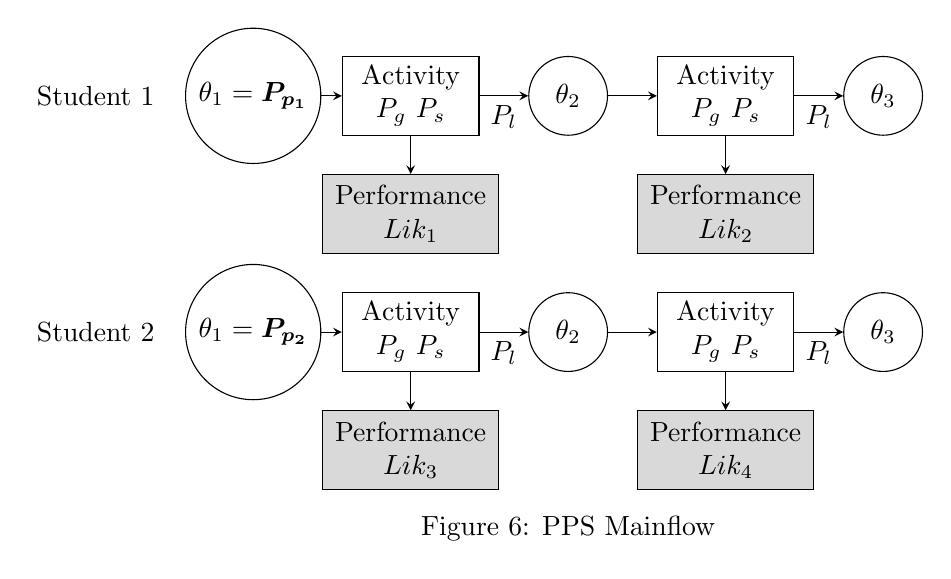
\begin{tikzpicture}
        % Define styles
        \tikzset{
            state/.style={circle, draw, minimum size=1cm},
            activity/.style={rectangle, draw, minimum size=1cm},
            performance/.style={rectangle, draw, fill=gray!30, minimum size=1cm},
            arrow/.style={->,>=stealth}
        }
        
        % Nodes
        \node[] () at (-2,0) {Student 1};
        \node[state] (state_node_1) at (0,0) {$\theta_1 = \boldsymbol{P_{p_1}}$};
        \node[activity] (activity_node_1) at (2,0) {\parbox{1.5cm}{\centering Activity \\ $P_g \ P_s$}};
        \node[performance] (performance_node_1) at (2,-1.5) {\parbox{2cm}{\centering Performance \\ $Lik_1$}};
        \node[state] (state_node_2) at (4,0) {$\theta_2$};
        
        \node[activity] (activity_node_2) at (6,0) {\parbox{1.5cm}{\centering Activity \\ $P_g \ P_s$}};
        \node[performance] (performance_node_2) at (6,-1.5) {\parbox{2cm}{\centering Performance \\ $Lik_2$}};
        \node[state] (state_node_3) at (8,0) {$\theta_3$};
        
        % Arrows
        \draw[arrow] (state_node_1) -- (activity_node_1);
        \draw[arrow] (activity_node_1) -- (state_node_2) node[midway, below] {$P_l$};
        \draw[arrow] (activity_node_1) -- (performance_node_1);
        \draw[arrow] (state_node_2) -- (activity_node_2);
        \draw[arrow] (activity_node_2) -- (state_node_3) node[midway, below] {$P_l$};
        \draw[arrow] (activity_node_2) -- (performance_node_2);
    

        % student 2
        \node[] () at (-2,-3) {Student 2};
        \node[state] (state_node_2) at (0,-3) {$\theta_1 = \boldsymbol{P_{p_2}}$};
        \node[activity] (activity_node_2) at (2,-3) {\parbox{1.5cm}{\centering Activity \\ $P_g \ P_s$}};
        \node[performance] (performance_node_2) at (2,-4.5) {\parbox{2cm}{\centering Performance \\ $Lik_3$}};
        \node[state] (state_node_3) at (4,-3) {$\theta_2$};
        \node[activity] (activity_node_3) at (6,-3) {\parbox{1.5cm}{\centering Activity \\ $P_g \ P_s$}};
        \node[performance] (performance_node_3) at (6,-4.5) {\parbox{2cm}{\centering Performance \\ $Lik_4$}};
        \node[state] (state_node_4) at (8,-3) {$\theta_3$};
        \draw[arrow] (state_node_2) -- (activity_node_2);
        \draw[arrow] (activity_node_2) -- (state_node_3) node[midway, below] {$P_l$};
        \draw[arrow] (activity_node_2) -- (performance_node_2);
        \draw[arrow] (state_node_3) -- (activity_node_3);
        \draw[arrow] (activity_node_3) -- (state_node_4) node[midway, below] {$P_l$};
        \draw[arrow] (activity_node_3) -- (performance_node_3);

        % Footnote
        \node at (4,-5.5) {Figure 6: PPS Mainflow};
    \end{tikzpicture}
\end{center}

\subsubsection{Multiple Learn}

The Item Learning Effect (ILE) Model (\cite{multilearn}) is based on BKT that focuses on individualizing the learning rate. The BKT assumes all item (activity) share same learning rate, the global parameter \( P_l \). The ILE localizes learning rate into each item.

The main difference in the model description lies in the learning rate.

For each activity \( j \), let \( P_{l_j} \) denotes the learning rate.

The mainflow of ILE is illustrated in Figure 7. Note there are three different activities, 1, 2 and 3.

\begin{center}
    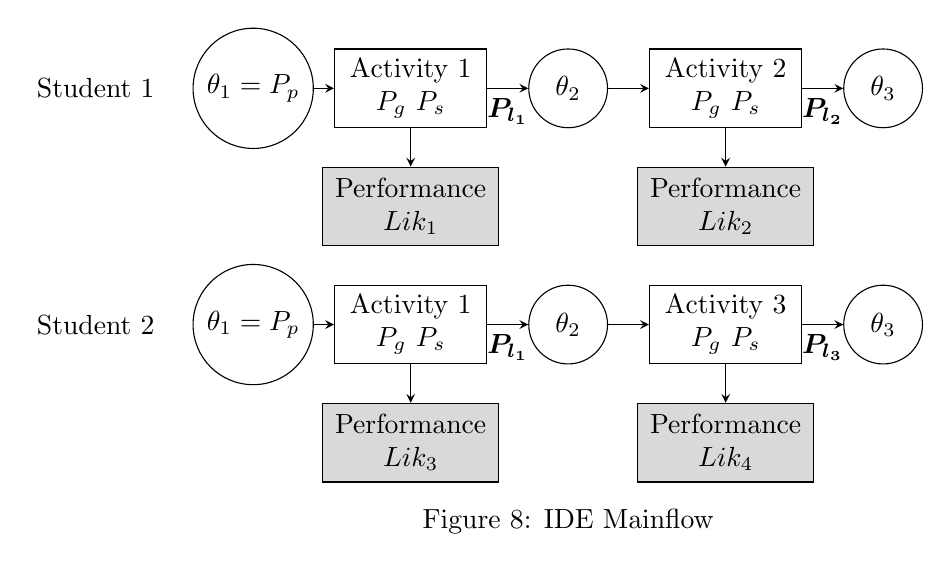
\begin{tikzpicture}
        % Define styles
        \tikzset{
            state/.style={circle, draw, minimum size=1cm},
            activity/.style={rectangle, draw, minimum size=1cm},
            performance/.style={rectangle, draw, fill=gray!30, minimum size=1cm},
            arrow/.style={->,>=stealth}
        }
        
        % Nodes
        \node[] () at (-2,0) {Student 1};
        \node[state] (state_node_1) at (0,0) {$\theta_1 = P_p$};
        \node[activity] (activity_node_1) at (2,0) {\parbox{1.7cm}{\centering Activity 1 \\ ${P_{g} \ P_{s}}$}};
        \node[performance] (performance_node_1) at (2,-1.5) {\parbox{2cm}{\centering Performance \\ $Lik_1$}};
        \node[state] (state_node_2) at (4,0) {$\theta_2$};
        
        \node[activity] (activity_node_2) at (6,0) {\parbox{1.7cm}{\centering Activity 2 \\ ${P_{g} \ P_{s}}$}};
        \node[performance] (performance_node_2) at (6,-1.5) {\parbox{2cm}{\centering Performance \\ $Lik_2$}};
        \node[state] (state_node_3) at (8,0) {$\theta_3$};
        
        % Arrows
        \draw[arrow] (state_node_1) -- (activity_node_1);
        \draw[arrow] (activity_node_1) -- (state_node_2) node[midway, below] {$\boldsymbol{P_{l_1}}$};
        \draw[arrow] (activity_node_1) -- (performance_node_1);
        \draw[arrow] (state_node_2) -- (activity_node_2);
        \draw[arrow] (activity_node_2) -- (state_node_3) node[midway, below] {$\boldsymbol{P_{l_2}}$};
        \draw[arrow] (activity_node_2) -- (performance_node_2);
    

        % student 2
        \node[] () at (-2,-3) {Student 2};
        \node[state] (state_node_2) at (0,-3) {$\theta_1 = P_p$};
        \node[activity] (activity_node_2) at (2,-3) {\parbox{1.7cm}{\centering Activity 1 \\ ${P_{g} \ P_{s}}$}};
        \node[performance] (performance_node_2) at (2,-4.5) {\parbox{2cm}{\centering Performance \\ $Lik_3$}};
        \node[state] (state_node_3) at (4,-3) {$\theta_2$};
        \node[activity] (activity_node_3) at (6,-3) {\parbox{1.7cm}{\centering Activity 3 \\ ${P_{g} \ P_{s}}$}};
        \node[performance] (performance_node_3) at (6,-4.5) {\parbox{2cm}{\centering Performance \\ $Lik_4$}};
        \node[state] (state_node_4) at (8,-3) {$\theta_3$};
        \draw[arrow] (state_node_2) -- (activity_node_2);
        \draw[arrow] (activity_node_2) -- (state_node_3) node[midway, below] {$\boldsymbol{P_{l_1}}$};
        \draw[arrow] (activity_node_2) -- (performance_node_2);
        \draw[arrow] (state_node_3) -- (activity_node_3);
        \draw[arrow] (activity_node_3) -- (state_node_4) node[midway, below] {$\boldsymbol{P_{l_3}}$};
        \draw[arrow] (activity_node_3) -- (performance_node_3);

        % Footnote
        \node at (4,-5.5) {Figure 8: IDE Mainflow};
    \end{tikzpicture}
\end{center}


\subsubsection{Multiple Pair}

The Item Order Effect (IOE) Model (\cite{multipair}) is based on BKT that focuses on individualizing the learning rate. The BKT assumes all item (activity) share same learning rate, the global parameter \( P_l \). The IOE localizes learning rate into each item pairs.

The main difference in the model description lies in the learning rate.

For each activity \( i \) and activity \( j \), let \( P_{l_{ij}} \) denotes the learning rate from activity \( i \) to activity \( j \). Note \( P_{l_{0j}} \) refers initial activity learn rate.

The mainflow of ILE is illustrated in Figure 9. Note there are three different activities, 1, 2 and 3 with most 6 pairs.

\begin{center}
    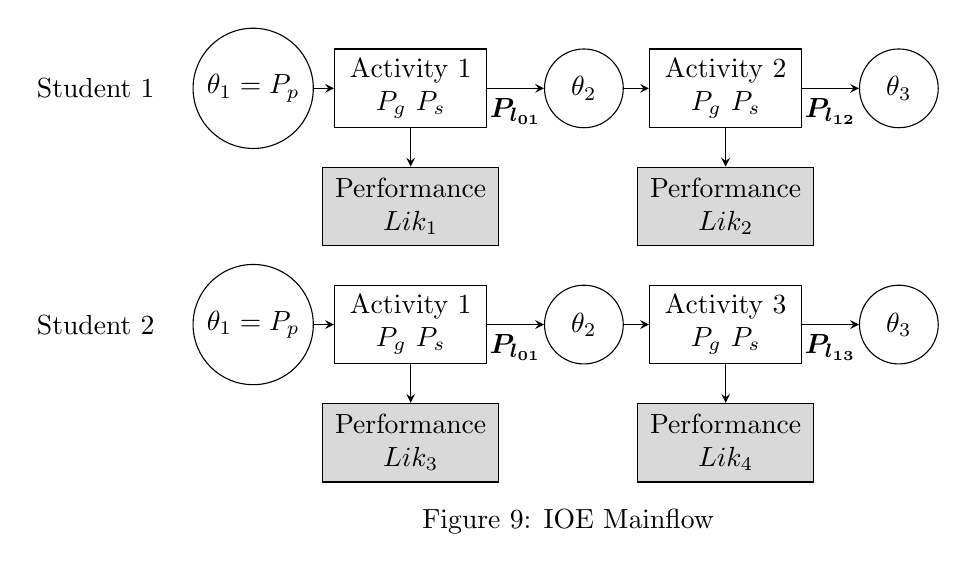
\begin{tikzpicture}
        % Define styles
        \tikzset{
            state/.style={circle, draw, minimum size=1cm},
            activity/.style={rectangle, draw, minimum size=1cm},
            performance/.style={rectangle, draw, fill=gray!30, minimum size=1cm},
            arrow/.style={->,>=stealth}
        }
        
        % Nodes
        \node[] () at (-2,0) {Student 1};
        \node[state] (state_node_1) at (0,0) {$\theta_1 = P_p$};
        \node[activity] (activity_node_1) at (2,0) {\parbox{1.7cm}{\centering Activity 1 \\ ${P_{g} \ P_{s}}$}};
        \node[performance] (performance_node_1) at (2,-1.5) {\parbox{2cm}{\centering Performance \\ $Lik_1$}};
        \node[state] (state_node_2) at (4.2,0) {$\theta_2$};
        
        \node[activity] (activity_node_2) at (6,0) {\parbox{1.7cm}{\centering Activity 2 \\ ${P_{g} \ P_{s}}$}};
        \node[performance] (performance_node_2) at (6,-1.5) {\parbox{2cm}{\centering Performance \\ $Lik_2$}};
        \node[state] (state_node_3) at (8.2,0) {$\theta_3$};
        
        % Arrows
        \draw[arrow] (state_node_1) -- (activity_node_1);
        \draw[arrow] (activity_node_1) -- (state_node_2) node[midway, below] {$\boldsymbol{P_{l_{01}}}$};
        \draw[arrow] (activity_node_1) -- (performance_node_1);
        \draw[arrow] (state_node_2) -- (activity_node_2);
        \draw[arrow] (activity_node_2) -- (state_node_3) node[midway, below] {$\boldsymbol{P_{l_{12}}}$};
        \draw[arrow] (activity_node_2) -- (performance_node_2);
    

        % student 2
        \node[] () at (-2,-3) {Student 2};
        \node[state] (state_node_2) at (0,-3) {$\theta_1 = P_p$};
        \node[activity] (activity_node_2) at (2,-3) {\parbox{1.7cm}{\centering Activity 1 \\ ${P_{g} \ P_{s}}$}};
        \node[performance] (performance_node_2) at (2,-4.5) {\parbox{2cm}{\centering Performance \\ $Lik_3$}};
        \node[state] (state_node_3) at (4.2,-3) {$\theta_2$};
        \node[activity] (activity_node_3) at (6,-3) {\parbox{1.7cm}{\centering Activity 3 \\ ${P_{g} \ P_{s}}$}};
        \node[performance] (performance_node_3) at (6,-4.5) {\parbox{2cm}{\centering Performance \\ $Lik_4$}};
        \node[state] (state_node_4) at (8.2,-3) {$\theta_3$};
        \draw[arrow] (state_node_2) -- (activity_node_2);
        \draw[arrow] (activity_node_2) -- (state_node_3) node[midway, below] {$\boldsymbol{P_{l_{01}}}$};
        \draw[arrow] (activity_node_2) -- (performance_node_2);
        \draw[arrow] (state_node_3) -- (activity_node_3);
        \draw[arrow] (activity_node_3) -- (state_node_4) node[midway, below] {$\boldsymbol{P_{l_{13}}}$};
        \draw[arrow] (activity_node_3) -- (performance_node_3);

        % Footnote
        \node at (4,-5.5) {Figure 9: IOE Mainflow};
    \end{tikzpicture}
\end{center}


\subsubsection{Multiple Guess and Slip}

The Item Difficulty Effect (IDE) Model (\cite{multiguess}) is based on BKT that focuses on individualizing the guess and slip. The BKT assumes all item (activity) share same guess and slip rate, the global parameter \( P_g \) and \( P_s \). The IDE localizes guess and slip rate into each item.

The main difference in the model description lies in the guess and slip rate.

For each activity \( j \), let \( P_{g_j} \) denotes the guess rate and \( P_{s_j} \) denotes the slip rate.

The mainflow of PPS is illustrated in Figure 10. Note there are three different activities, 1, 2 and 3.

\begin{center}
    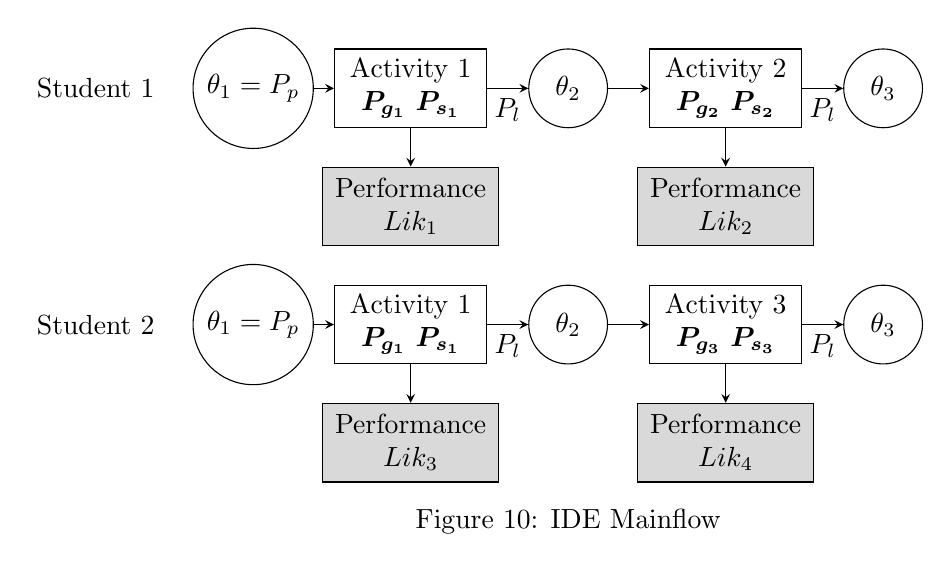
\begin{tikzpicture}
        % Define styles
        \tikzset{
            state/.style={circle, draw, minimum size=1cm},
            activity/.style={rectangle, draw, minimum size=1cm},
            performance/.style={rectangle, draw, fill=gray!30, minimum size=1cm},
            arrow/.style={->,>=stealth}
        }
        
        % Nodes
        \node[] () at (-2,0) {Student 1};
        \node[state] (state_node_1) at (0,0) {$\theta_1 = P_p$};
        \node[activity] (activity_node_1) at (2,0) {\parbox{1.7cm}{\centering Activity 1 \\ $\boldsymbol{P_{g_1} \ P_{s_1}}$}};
        \node[performance] (performance_node_1) at (2,-1.5) {\parbox{2cm}{\centering Performance \\ $Lik_1$}};
        \node[state] (state_node_2) at (4,0) {$\theta_2$};
        
        \node[activity] (activity_node_2) at (6,0) {\parbox{1.7cm}{\centering Activity 2 \\ $\boldsymbol{P_{g_2} \ P_{s_2}}$}};
        \node[performance] (performance_node_2) at (6,-1.5) {\parbox{2cm}{\centering Performance \\ $Lik_2$}};
        \node[state] (state_node_3) at (8,0) {$\theta_3$};
        
        % Arrows
        \draw[arrow] (state_node_1) -- (activity_node_1);
        \draw[arrow] (activity_node_1) -- (state_node_2) node[midway, below] {$P_l$};
        \draw[arrow] (activity_node_1) -- (performance_node_1);
        \draw[arrow] (state_node_2) -- (activity_node_2);
        \draw[arrow] (activity_node_2) -- (state_node_3) node[midway, below] {$P_l$};
        \draw[arrow] (activity_node_2) -- (performance_node_2);
    

        % student 2
        \node[] () at (-2,-3) {Student 2};
        \node[state] (state_node_2) at (0,-3) {$\theta_1 = P_p$};
        \node[activity] (activity_node_2) at (2,-3) {\parbox{1.7cm}{\centering Activity 1 \\ $\boldsymbol{P_{g_1} \ P_{s_1}}$}};
        \node[performance] (performance_node_2) at (2,-4.5) {\parbox{2cm}{\centering Performance \\ $Lik_3$}};
        \node[state] (state_node_3) at (4,-3) {$\theta_2$};
        \node[activity] (activity_node_3) at (6,-3) {\parbox{1.7cm}{\centering Activity 3 \\ $\boldsymbol{P_{g_3} \ P_{s_3}}$}};
        \node[performance] (performance_node_3) at (6,-4.5) {\parbox{2cm}{\centering Performance \\ $Lik_4$}};
        \node[state] (state_node_4) at (8,-3) {$\theta_3$};
        \draw[arrow] (state_node_2) -- (activity_node_2);
        \draw[arrow] (activity_node_2) -- (state_node_3) node[midway, below] {$P_l$};
        \draw[arrow] (activity_node_2) -- (performance_node_2);
        \draw[arrow] (state_node_3) -- (activity_node_3);
        \draw[arrow] (activity_node_3) -- (state_node_4) node[midway, below] {$P_l$};
        \draw[arrow] (activity_node_3) -- (performance_node_3);

        % Footnote
        \node at (4,-5.5) {Figure 10: IDE Mainflow};
    \end{tikzpicture}
\end{center}


\subsubsection{Forget}

The learning and forgetting behavior (LFB) Model (\cite{forget}) is based on BKT that consider forgetting as part of learning process. The LFB assumes that 

The main difference in the model description lies in the state changes.Besides original three types of learning state changes (Remaining Known, Learning, Remaining Unknown), LFB adds Forget which is illustrated in Figure 11.

\begin{center}
    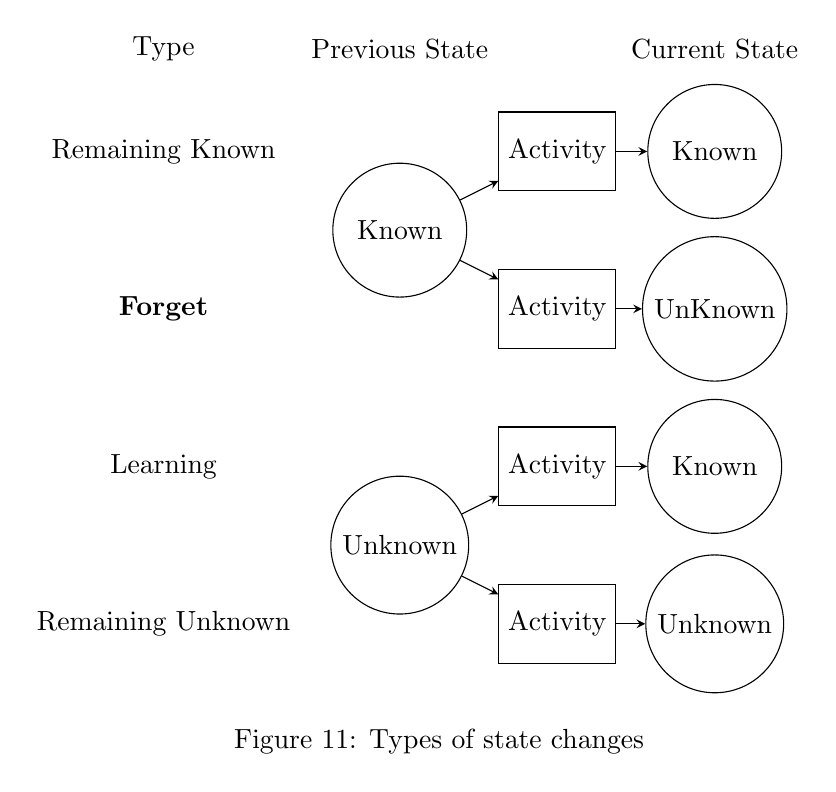
\begin{tikzpicture}
        % Define styles
        \tikzset{
            state/.style={circle, draw, minimum size=1.7cm},
            activity/.style={rectangle, draw, minimum size=1cm},
            arrow/.style={->,>=stealth}
        }
        
        % Nodes
        \node[] () at (-3,3.3) {Type};
        \node[] () at (0,3.3) {Previous State};
        \node[] () at (4,3.3) {Current State};

        \node[] () at (-3,2) {Remaining Known};
        \node[state] (state_node_1) at (0,1) {Known};
        \node[activity] (activity_node_1) at (2,2) {Activity};
        \node[state] (state_node_2) at (4,2) {Known};

        \node[] () at (-3,0) {\textbf{Forget}};
        \node[activity] (activity_node_0) at (2,0) {Activity};
        \node[state] (state_node_0) at (4,0) {UnKnown};
        
        \node[] () at (-3,-2) {Learning};
        \node[state] (state_node_3) at (0,-3) {Unknown};
        \node[activity] (activity_node_2) at (2,-2) {Activity};
        \node[state] (state_node_4) at (4,-2) {Known};
        
        \node[] () at (-3,-4) {Remaining Unknown};
        % \node[state] (state_node_5) at (0,-4) {Unknown};
        \node[activity] (activity_node_3) at (2,-4) {Activity};
        \node[state] (state_node_6) at (4,-4) {Unknown};
        
        % Arrows
        \draw[arrow] (state_node_1) -- (activity_node_1);
        \draw[arrow] (state_node_1) -- (activity_node_0);
        \draw[arrow] (activity_node_1) -- (state_node_2);
        \draw[arrow] (activity_node_0) -- (state_node_0);
        \draw[arrow] (state_node_3) -- (activity_node_2);
        \draw[arrow] (activity_node_2) -- (state_node_4);
        \draw[arrow] (state_node_3) -- (activity_node_3);
        \draw[arrow] (activity_node_3) -- (state_node_6);
    
        % Footnote
        \node at (0.5,-5.5) {Figure 11: Types of state changes};
    \end{tikzpicture}
\end{center}

In LFB terminology, we add the following defines:

1. \textbf{Forget}  
The forget rate, \( P_f \), represents the probability that a learner transitions to the unknown state through forgetting.

LFB Updates \(\theta_{i+1}\) by incorporating the potential learning effect based on \(\theta'\) in a different way with BKT, considering the effect of forget change.

$$
\theta_{i+1} = \theta' \boldsymbol{P_f} + (1 - \theta') P_l    
$$

The mainflow of LFB is illustrated in Figure 10. Note there are forget parameters $P_f$ in use.

\begin{center}
    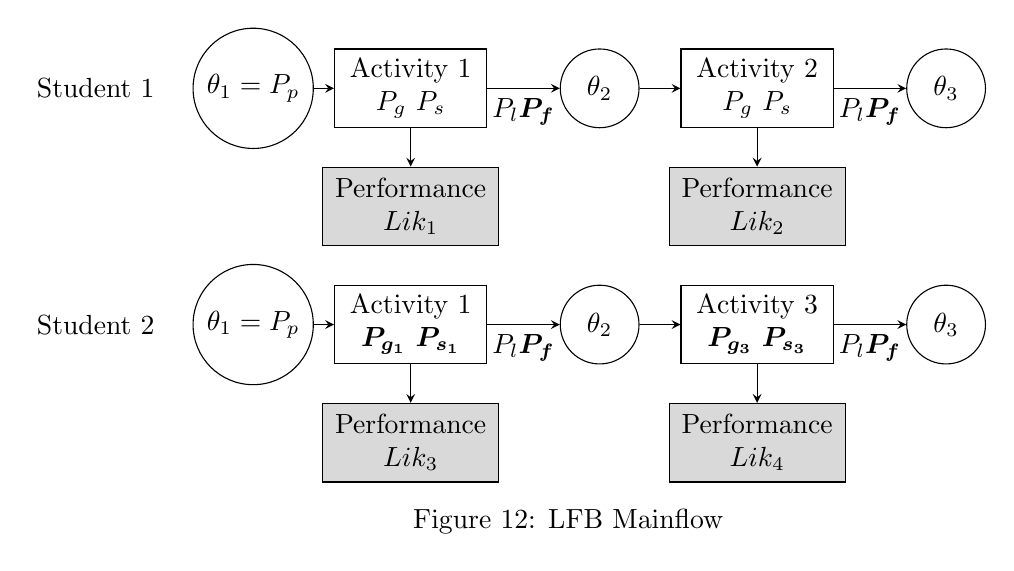
\begin{tikzpicture}
        % Define styles
        \tikzset{
            state/.style={circle, draw, minimum size=1cm},
            activity/.style={rectangle, draw, minimum size=1cm},
            performance/.style={rectangle, draw, fill=gray!30, minimum size=1cm},
            arrow/.style={->,>=stealth}
        }
        
        % Nodes
        \node[] () at (-2,0) {Student 1};
        \node[state] (state_node_1) at (0,0) {$\theta_1 = P_p$};
        \node[activity] (activity_node_1) at (2,0) {\parbox{1.7cm}{\centering Activity 1 \\ ${P_{g} \ P_{s}}$}};
        \node[performance] (performance_node_1) at (2,-1.5) {\parbox{2cm}{\centering Performance \\ $Lik_1$}};
        \node[state] (state_node_2) at (4.4,0) {$\theta_2$};
        
        \node[activity] (activity_node_2) at (6.4,0) {\parbox{1.7cm}{\centering Activity 2 \\ ${P_{g} \ P_{s}}$}};
        \node[performance] (performance_node_2) at (6.4,-1.5) {\parbox{2cm}{\centering Performance \\ $Lik_2$}};
        \node[state] (state_node_3) at (8.8,0) {$\theta_3$};
        
        % Arrows
        \draw[arrow] (state_node_1) -- (activity_node_1);
        \draw[arrow] (activity_node_1) -- (state_node_2) node[midway, below] {$P_l \boldsymbol{P_f}$};
        \draw[arrow] (activity_node_1) -- (performance_node_1);
        \draw[arrow] (state_node_2) -- (activity_node_2);
        \draw[arrow] (activity_node_2) -- (state_node_3) node[midway, below] {$P_l \boldsymbol{P_f}$};
        \draw[arrow] (activity_node_2) -- (performance_node_2);
    

        % student 2
        \node[] () at (-2,-3) {Student 2};
        \node[state] (state_node_2) at (0,-3) {$\theta_1 = P_p$};
        \node[activity] (activity_node_2) at (2,-3) {\parbox{1.7cm}{\centering Activity 1 \\ $\boldsymbol{P_{g_1} \ P_{s_1}}$}};
        \node[performance] (performance_node_2) at (2,-4.5) {\parbox{2cm}{\centering Performance \\ $Lik_3$}};
        \node[state] (state_node_3) at (4.4,-3) {$\theta_2$};
        \node[activity] (activity_node_3) at (6.4,-3) {\parbox{1.7cm}{\centering Activity 3 \\ $\boldsymbol{P_{g_3} \ P_{s_3}}$}};
        \node[performance] (performance_node_3) at (6.4,-4.5) {\parbox{2cm}{\centering Performance \\ $Lik_4$}};
        \node[state] (state_node_4) at (8.8,-3) {$\theta_3$};
        \draw[arrow] (state_node_2) -- (activity_node_2);
        \draw[arrow] (activity_node_2) -- (state_node_3) node[midway, below] {$P_l \boldsymbol{P_f}$};
        \draw[arrow] (activity_node_2) -- (performance_node_2);
        \draw[arrow] (state_node_3) -- (activity_node_3);
        \draw[arrow] (activity_node_3) -- (state_node_4) node[midway, below] {$P_l \boldsymbol{P_f}$};
        \draw[arrow] (activity_node_3) -- (performance_node_3);

        % Footnote
        \node at (4,-5.5) {Figure 12: LFB Mainflow};
    \end{tikzpicture}
\end{center}

% Reference
\printbibliography

\end{document}
